%% ----------------------------------------------------------------
%% Thesis.tex -- MAIN FILE (the one that you compile with LaTeX)
%% ---------------------------------------------------------------- 

% Set up the document
\documentclass[a4paper, 13pt, oneside]{Thesis}  % Use the "Thesis" style, based on the ECS Thesis style by Steve Gunn
\graphicspath{Figures/}  % Location of the graphics files (set up for graphics to be in PDF format)

% Include any extra LaTeX packages required
\usepackage[square, numbers, comma, sort&compress]{natbib}  % Use the "Natbib" style for the references in the Bibliography
\usepackage{verbatim}  % Needed for the "comment" environment to make LaTeX comments
\usepackage{vector}  % Allows "\bvec{}" and "\buvec{}" for "blackboard" style bold vectors in maths
\usepackage{graphicx}
\graphicspath{ {images/} }
\usepackage{array}
\usepackage{mathtools}
\usepackage{listings}
\usepackage{color}

\definecolor{dkgreen}{rgb}{0,0.6,0}
\definecolor{gray}{rgb}{0.5,0.5,0.5}
\definecolor{mauve}{rgb}{0.58,0,0.82}

\lstset{frame=tb,
  language=Java,
  aboveskip=3mm,
  belowskip=3mm,
  showstringspaces=false,
  columns=flexible,
  basicstyle={\small\ttfamily},
  numbers=none,
  numberstyle=\tiny\color{gray},
  keywordstyle=\color{blue},
  commentstyle=\color{dkgreen},
  stringstyle=\color{mauve},
  breaklines=true,
  breakatwhitespace=true,
  tabsize=3
}

\hypersetup{urlcolor=blue, colorlinks=true}  % Colours hyperlinks in blue, but this can be distracting if there are many links.

%% ----------------------------------------------------------------
\begin{document}
\frontmatter      % Begin Roman style (i, ii, iii, iv...) page numbering

% Set up the Title Page
\title  {AN APPLICATION OF AUDIO DATA HIDING: RADIO BROADCAST AS
A HIGH UTILITY SERVICE}
\authors  {\texorpdfstring
            {\href{nttin@apcs.vn}{TRONG-TIN NGUYEN - 1251045}}
            {Author Name}
            }
\addresses  {\groupname\\\deptname\\\univname}  % Do not change this here, instead these must be set in the "Thesis.cls" file, please look through it instead
\date       {HO CHI MINH CITY, 2016}
\subject    {}
\keywords   {}

\maketitle
%% ----------------------------------------------------------------

\setstretch{1.5}  % It is better to have smaller font and larger line spacing than the other way round

% Define the page headers using the FancyHdr package and set up for one-sided printing
\fancyhead{}  % Clears all page headers and footers
\rhead{\thepage}  % Sets the right side header to show the page number
\lhead{}  % Clears the left side page header

\pagestyle{fancy}  % Finally, use the "fancy" page style to implement the FancyHdr headers

%% ----------------------------------------------------------------
% Declaration Page required for the Thesis, your institution may give you a different text to place here
%% ----------------------------------------------------------------
% The "Funny Quote Page"
%% ----------------------------------------------------------------
%% ----------------------------------------------------------------

\setstretch{1.5}  % Reset the line-spacing to 1.3 for body text (if it has changed)

% The Acknowledgements page, for thanking everyone
\acknowledgements{
\addtocontents{toc}{\vspace{1em}}  % Add a gap in the Contents, for aesthetics

To be completely honest, it is impossible for me to complete this thesis without the guidance, support, help and encouragement of many people. I would like to express my sincerity towards all those who sail with me on this boat.

I would like to thank my thesis advisor, Dr. Minh-Nhut Ngo whose guidance and support had assisted me at all time regardless of time and difficulty. I truly appreciate the advices, discussion and encouragement that Dr. Minh-Nhut Ngo had given me during my thesis project. His great knowledge in this particular field is extremely valuable for me to open up ideas and solution. Last but not least, his dedication in our work is the source of motivation for me through the entire 9 months of the project.

I would like to thank all of my classmates and colleagues whose support had given me encouragement to finish this project. Although they may not involve in the professional terms, it is the joy that they bring to me that I feel refreshed and can continue to focus in the project

Most importantly, I would like to express gratitude for my family for their unconditional support and love. I could not complete this thesis without the people that are closest to me.	

}
\clearpage  % End of the Acknowledgements
%% ----------------------------------------------------------------
%% ----------------------------------------------------------------
\lhead{\emph{Contents}}  % Set the left side page header to "Contents"
\tableofcontents  % Write out the Table of Contents

%% ----------------------------------------------------------------

%% ----------------------------------------------------------------
\lhead{\emph{List of Figures}}  % Set the left side page header to "List if Figures"
\listoffigures  % Write out the List of Figures

%% ----------------------------------------------------------------
\lhead{\emph{List of Tables}}  % Set the left side page header to "List of Tables"
\listoftables  % Write out the List of Tables

\setstretch{1.5}  % Set the line spacing to 1.5, this makes the following tables easier to read
\clearpage  % Start a new page
\lhead{\emph{}}  % Set the left side page header to "Abbreviations"
\listofsymbols{ll}  % Include a list of Abbreviations (a table of two columns)
{
% \textbf{Acronym} & \textbf{W}hat (it) \textbf{S}tands \textbf{F}or \\
\textbf{BDR} & \textbf{B}it \textbf{D}etection \textbf{R}ate \\
\textbf{DPC} & \textbf{D}ynamic \textbf{P}hase \textbf{C}oding \\
\textbf{DSP} & \textbf{D}igital \textbf{S}ignal \textbf{P}rocessing \\
\textbf{FFT} & \textbf{F}ast \textbf{F}ourier \textbf{T}ransform \\
\textbf{IIR} & \textbf{I}finite \textbf{I}mpulse \textbf{R}esponse \\
\textbf{IFFT} & \textbf{I}nverse \textbf{F}ast \textbf{F}ourier \textbf{T}ransform \\
\textbf{LSB} & \textbf{L}east \textbf{S}ignificant \textbf{B}it\\
\textbf{ODG} & \textbf{O}bjective \textbf{D}ifference \textbf{G}rade \\
\textbf{PEAQ} & \textbf{P}erceptial \textbf{E}valuation of \textbf{A}udio \textbf{Q}uality \\
\textbf{QIM} & \textbf{Q}uantization \textbf{I}ndex \textbf{M}odulation \\
\textbf{SPC} & \textbf{S}tatic \textbf{P}hase \textbf{C}oding \\
\textbf{SS} & \textbf{S}pread \textbf{S}pectrum\\
}
\clearpage  % End of the Acknowledgements

% The Abstract Page
\addtotoc{Abstract}  % Add the "Abstract" page entry to the Contents
\abstract{


\addtocontents{toc}{\vspace{1em}}  % Add a gap in the Contents, for aesthetics
The dramatic growth of Internet has been flourishing many new areas in the multimedia industry. Internet radio broadcasting is one of the fast expanding business that has been attracting a consistent amount of audience and publishers. According to many annual media reports, the growth of Internet radio broadcasting is boosted constantly and is predicted to continue with this rate. As the industry booms in capacity, the space of potential customers also widen. Other businesses would try to capitalize on this client base. And this is done by advertising on Internet radio.

Internet radio advertisements take the form as a normal audio advertisement played in between songs or broadcasting session. Inside the advertisement, information about the product is described as clear and concise as possible. However, it is known that lone audio information lacks the details that are not suitable to put inside the audio advertisement. Therefore, listeners often miss the surrounding information that help him know more about the product before decide whether he should invest more effort in the product. 

Because the Internet radio broadcasting produce output as mere stream of audio, is becames very hard to attach an package of extra information to the audio data to send to clients. If we modify the streaming standard and allow more data to be sent along with the audio data, only the client application that expect that kind of data would be able to catch our sent data.

Among many sciencific fields, audio data hiding has witnessed many greate improvements over the past few years. In this area, special codes are embedded into actual audio content without any affection to its normal use. Inspired by the interesting properties of audio data hiding, we aim to combine audio watermarking in our original problem to solve it.

The puropose of this project is to propose an audio streaming system that are capable of combining audio data hiding and audio streaming. So that, we can decorate the advertisement with extra information, increase it efficency in user engagement. The result show that this project did change and improve the way advertisement is served to listeners.
}

\clearpage  % Abstract ended, start a new page

%% ---------------------------------------------------------------

%% ----------------------------------------------------------------
\pagestyle{empty}  % No headers or footers for the following pages

\null\vfill
% Now comes the "Funny Quote", written in italics
\textit{``If you want to go fast, go alone. If you want to go far, go together.''}

\begin{flushright}
African Proverb.
\end{flushright}

\vfill\vfill\vfill\vfill\vfill\vfill\null
\clearpage  % Funny Quote page ended, start a new page

%% ----------------------------------------------------------------
\mainmatter	  % Begin normal, numeric (1,2,3...) page numbering
\pagestyle{fancy}  % Return the page headers back to the "fancy" style

% Include the chapters of the thesis, as separate files
% Just uncomment the lines as you write the chapters

\chapter{Introduction}
\section{Importance of research}
Recent advancement in technology in general has led to the flourishment of many undiscovered industries. Many of them involve with the rapid expansion of the Internet, as an effective channel to reach customers. One of these newcomers is Internet radio broadcasting. For the past 2 years, internet radio has been becoming a new mainstream form of entertainment that attracts a consistent amount 
of listeners and broadcasters. 
\begin{figure}[h]
	\centering
\includegraphics[width=\textwidth]{monthly-online-listening}
 	\caption{Monthly Online Listening. Source\cite{edisonslide}}
 	\label{fig:MonthlyOnlineListening}
\end{figure}
According to Infinite Dial report from Edison Reasearch\cite{edison2016}, the monthly internet radio audience has been constantly increasing for the last 15 years. In 2016, it passed over 50\% the total population that over 12 years old of the U.S, reached 57\%. This fact indicates a undeniable trend in the listening behavior of audience, that there are estimated 155 million people that listen to Internet radio monthly in America. 

In 2016, the reports from the same organization also show interesting data about the number of weekly Internet radio listeners, which rises from 44\% in 2015 to 50\% of respondents age 12 and older in 2016. With 57\% of Americans using online radio monthly in 2016, we can induce to the interesting fact that 88\% of them has made it a weekly habit, this is shown in details in \ref{fig:MonthlyWeekly}. 

From the same report, it tells that Internet radio listening now
averages about 12 hours and 53 minutes per week across
the weekly online radio listeners population in 2015. Listening hours are critical. They
represent opportunities to reach real people with
advertising messages. While according to the XappMedia Internet Radio Ad Load Report in Quater 1 of 2015\cite{xapp2015q1}, it revealed an average of 2 minutes and 18 seconds of ads
per hour. At 12:53 hours of listening per week, that reflects
about 29 minutes of ads. Recent analysis shows the
average Internet radio spot length is 25.88 seconds, which
translates into about 68 ad impressions per week, per
listener. 

It is also reported that 95\% of the audience choose ad-supported listening form. That domination opens a huge number of opportunities for advertisers to reach an engaged audience. In fact, internet radio advertising is the new trend with findings from the Internet Radio Ad Load Report Q4 2015\cite{xapp2015q4}, where the total advertisers indentified through 2015 rose to 406, a 5.4x increase over 2014. This form of advertising plays fewer commercials per hour, which result in higher listener attention levels, increasing the ads, intended effect. Plus, listeners are only one click away from an advertiser's web site. They are online and have browser window open. This makes it very easy to get listeners to visit the advertiser's website. Web radio listeners are also a highly active group of consumers with an above average level of purchase intention.


\begin{figure}[h]
	\centering
\includegraphics[width=\textwidth]{monthly-weekly}
 	\caption{Monthly online radio listeners who also listen weekly. Source\cite{edisonslide}}
 	\label{fig:MonthlyWeekly}
\end{figure}

For businesses, it is important to reaching out to as many clients as possible. To achieve this, one should capitalize on a type of marketing and focus on enhancing its effectiveness. In the case of internet radio, since it's a relatively new field, research is required to make the most advantage out of this new advertising form. Otherwise, a bad model would not last long due to the fast changing pace tech industry. In such a state, one has to equipped himself with knowledge and tools to be adaptable to different situations.

There are a lot of research one can try to strengthen his advertising system. He can either publish more channels leading to customers, make better content or invest more money into the campaign. For this particular project, we focus on a more scienctific approach, which of course has many trade offs compare to other ones. Open a research and development project, apply the knowledge into a live system are not easy, care must be taken very serisously when such decisions are made. It's important to take everything in the equation, where we can evaluate what's are the trade offs of our research. Otherwise, one might waste time and resources going the wrong path. 

In general, an enhancement in terms of science would question the existing system in a most fundamental way. It is totally possible that one has to replace his whole model for a scienctific solution to come in. And this takes times and a lot of effort. But on the other hand, since it focuses on the root of all causes, not just patching here and there, it would be able to solve classic puzzles that other approaches can not. 

To choose the right path, we should consider the context of our problem, the Internet itself. Rapidly changing in all dimensions, unpredictable and chaotic are the properties of the Internet nowadays. Common businesses are not equipped with necessary tools to deal with this. Therefore, they often find themselves solving problems that keep pops up one after another. Only a scienctific solution can help them in this battle.

\section{Challenges	with traditional radio advertising}

At the time of this research, the popular form of advertising over radio channel is done by inserting an advertising fragment into the streaming buffer. By this way, it produces a stream of media that plays out naturally with autual content separated by advertisements. 

There are many big multimedia streaming companies that use this approach, namely Spotify, Youtube or Apple Music. A good point with this method is its simplicity. Straightforwardly, temporarily pause the stream and play an advertisement until it ends or users explicitly skip. Simple means easy to deploy and get up and running, plug and play with different settings. That would help boost the market research progress or anything favor flash launching. An obvious downside is actively interupting user experience with advertisements. Unless it is a relevant one, user would feel annoyed and skip the advertisement or even leave the session. For established cooperation, they focus on the amount of advertisement views, not necessarily engagement quality, as they already have a tremendous userbase. Hence, this method apparently fits them.

However, for small project, listeners are very important so it's not wise to take risk degrading the user experience. Instead, the advertisement content should be made carefully too, to use as a tool to attract even more users. And this is not something traditional methods are really good at. Plus, there is a classic challenge that any form of advertisement face, it hardly creates any potential audience engagement that could lead to actual advertising success. The traditional system lacks a channel that effectively guide listeners to the advertisers intention rather than mere meaningless advertising audio. And this is what we are trying to solve.

\section {Motivation and Research Aims}

Seeing how promising the industry of Internet radio broadcasting is, it appears urgent that we should propose a systemic solution to help magnify the good points and minimize the bad points of this innovate channel. Internet radio advertising find itself good at providing a cheap way to reach listeners, while also possible to be effective if further consideration in advertising timing and content is made. On the other hand, one of its bad sides is lacking effectiveness in user engagement. In order to optimize this, we need the following points for our system:
\begin{itemize}
\item{On top of our solution, we want to reserve the benefits of traditional Internet radio advertising. That is cheap, simple and easy to implement.}
\item{A way to exhibit more relevant contents that support the advertisement. Traditional way of broadcasting advertisement lacks a space for that kind of extra information. While it appears naturally that pure audio ads are not enough to notice listeners. One might missheard the advertisement and has no way to go back, he has to go online to look for more information. Plus, it's better to have extra information supporting the running advertisement. Listener might want to research further information about pricing, extra options before deciding to buy products from advertisements.}
\end{itemize}

\section {Thesis Outline}
This thesis is comprised of six chapters. A schemantic overview of this thesis is shown in Fig. \ref{fig:ThesisOverview}. Chapters 2-6 are organized as follows.

Chapter 2 presents the background knowledge related to this thesis and the key principles for the proposed approach. It starts with an overview of our solution, then glimpse the needed parts that we need for this project. We also present in details the concepts that we borrow from other fields such as audio data hiding and concurrency programming.

Chapter 3  and 4 show our proposed method based on the background we had describe in Chapter 2. We divide our system into many small part, each with its own section to discuss. In the process, we also bring up many unresolved issues with some classic trade offs, which we rely on experimenting in Chapter 5 to deal with. To provide a intuitively walkthrough of our system, we exhibit many flow charts to resemble the system.

We continue to the testing, experimenting and optimzation in Chapter 5. While Chapter 4 points out several parameters we need to optimize, Chapter 5 propose and execute tests on different settings to determine the best choice. We then provide test results presented in meaningful figures, which would help us make sense of the data and choose our optimal solution. 

Finally, Chapter 6 summarizes this study, gives some concluding remarks, highlights our contributions to the advertising industry, and opens a number of directions for further upgrade to the system.

\begin{figure}
  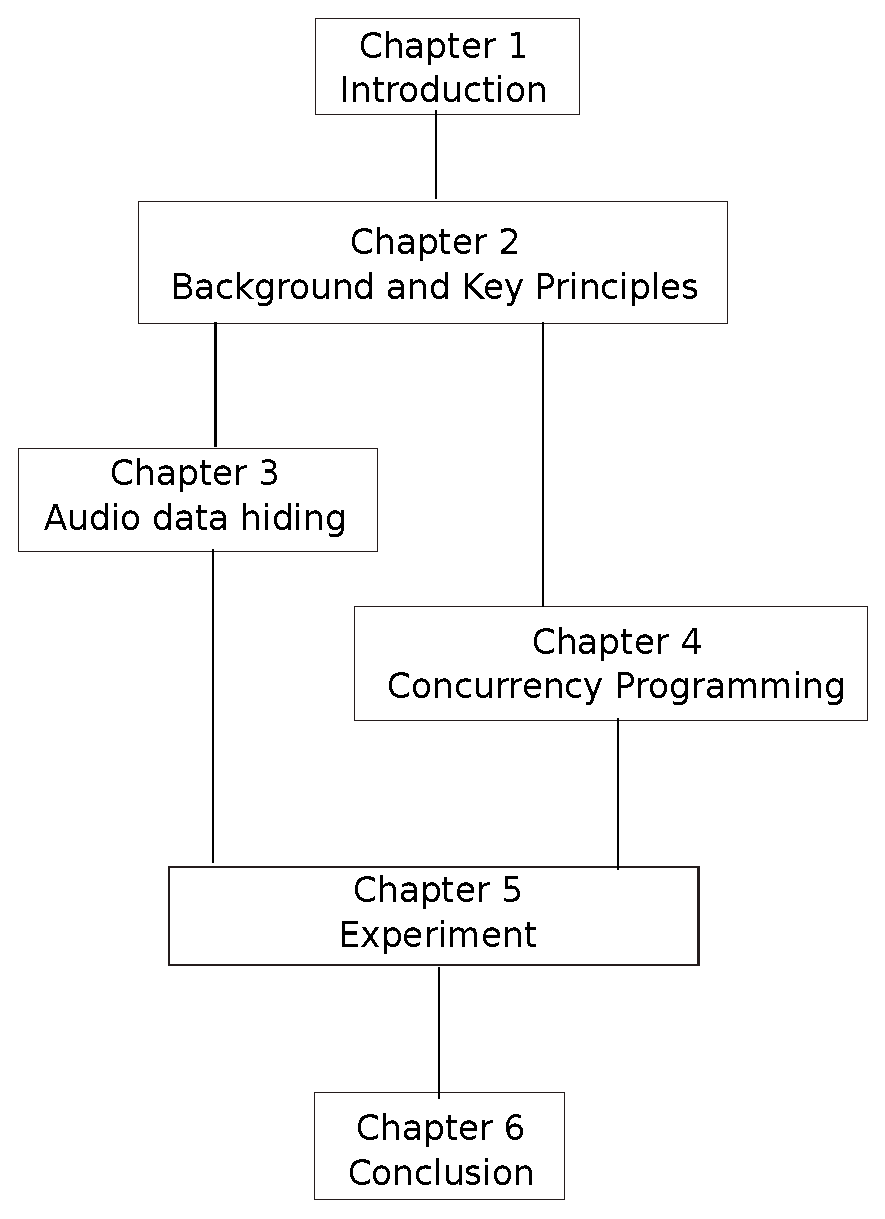
\includegraphics{drawing-2.eps}
  \caption{The schemantic overview of the thesis}
  \label{fig:ThesisOverview}
\end{figure} % Introduction

\chapter{Background and Key Principle}

\section{Overview of Audio Data Hiding}

\subsection {General Scheme}
Audio data hiding or audio watermarking is the process of embedding information into audio data. There are two phases in general: watermark embedding and watermark detection. For embedding, an information is embedded into a original audio signal, produced a watermarked audio signal. This signal is sent to many other source for consuming and might suffer from some kind of processing or attacks, which might degrade the audio quality or the embedded watermark's correctness. On the other hand, watermark detection uses a watermark detector to extract the inserted watermark.

Usually, the original signal is divided into frames with a fixed frame length, the reason for this action would be discussed later in the thesis. Watermark bits are embedded into those frames using embedding techniques. After that, all the frames would be combined together to create a watermarked audio data. Similarly, watermark detector also split data into frame with the same parameter framelength, and use an inverse version of embedding technique to extract watermark.

\subsection {Performance Evaluation}
The field of audio data hiding has been existed for about twenty years, resulting in a lot of different approaches. This section presents several important definition required for evaluating an audio data hiding method. Usually, perceptual evaluation of audio quality (PEAQ) is used to measure the sound quality of the watermarked signals. Bit detection rate (BDR) is used to measure the accuracy of watermarking detection process.
\subsubsection*{Perceptual evaluation of audio quality}
PEAQ is used to measure quality degradation in audio according to the objective difference grade (ODG) which ranges from −4 to 0. ODG indicates the sound quality of target signals as shown in Table \ref{tab:PEAQ}.


\begin{figure}
\begin{center}
\begin{tabular}{ | m{6cm} | m{1cm} | } 
\hline
Quality degradation & ODG \\ 
\hline
Imperceptible & 0 \\ 
\hline
Perceptible, but not annoying & -1 \\ 
\hline
Slightly annoying & -2 \\ 
\hline
Annoying & -3 \\ 
\hline
Very annoying & -4 \\ 
\hline
\end{tabular}
\caption{Quality degradation of sound and PEAQ (ODG).}
\label{tab:PEAQ}
\end{center}
\end{figure}


\subsubsection*{Detection accuracy}
Detection accuracy was measured by BDR, the ratio between the numbers of correct bits and total bits as follows.
\begin{align}
\mbox{BDR} = \frac{\mbox{number of correctly detected bits}}{\mbox{total number of bits}}
\end{align}

\subsection{Embedding Techniques}
\subsubsection*{Methods based on least significant bits}
Methods based on least significant bits are the most conventional and simple technique. Watermark is embedded into audio signals by substituting or
manipulating the LS-bits of audio samples according to watermark bits. Since LS-bits do
not have much effect to the quality of audio signal, the distortion caused by this method
is not severe, hence the watermark is inaudible to users. The other advantage is the high
bit rate, e.g., 44100 bps for audio signals with a sampling frequency of 44.1 kHz. However,
this method has a serious limitation with robustness, even against simple signal-processing
manipulation such as addition of white noise.


\subsubsection*{Methods based on spread spectrum}
Inspired from the concept used in spread spectrum (SS) communication, a number of
methods of audio data hiding based on spread spectrum have been proposed. The principle
is that the watermark is spread over the large bandwidth spectrum so that the energy in a
single frequency is very small and it can be undetectable. This also enables the watermark
to be easily detected even if there is interference on some frequencies.
\subsubsection*{Methods based on echo hiding}
The simplest method based on echo hiding embeds information into the host signal by
introducing an echo in the host signal, which is an annutated delayed version of the host
signal \cite{echohiding} The watermark is encoded by the delay time of the echo, e.g., two different
values of delay time are used to encode one watermark bit. The delay times are carefully
chosen so that the watermark is inaudible and recoverable. By optimzing the delay
time, adding the echo to the host signal essentially emphasizes the host signal, making it
perceived louder, hence the watermark is basically inaudible to human auditory system
(HAS)\cite{has}
\subsubsection*{Methods in transform domain}
Methods in transformed domain exploit advantages of simultaneous masking character-
istics of HAS to embed inaudible watermarks. It is easier to incorporate perceptual
knowledge into the embedding algorithm in transformed domain than in time domain. A
simple way of exploiting perceptual knowledge is to embed watermark into the mid-range
frequency component, since the low frequency components are more sensitive to noise
and the high frequency components can be remove without degrading the audio quality.
Also, many of the state-of-the-art compression techniques such as MP3\cite{mp3} work in the same
framework. Watermark can be adapted with the models to resist perceptual compression.

In general, quantization index modulation (QIM)\cite{qim} technique is used for embedding
watermark in transformed domain because of its good robustness and blind nature \cite{QIMtwice}.
The embedding rule is quite simple. Suppose that a watermark bit needs to be embedded
into a variable, QIM quantizes the value of this variable according to the corresponding
scale. The watermarked variable is transmitted and may suffer from noise. To detect, the
distance from the watermarked variable to its closet point in each scale are calculated and
the watermark bit is decided by choosing the bit corresponding to the scale with the lower
distance. When applied to audio watermarking, QIM needs to specific acoustic features,
e.g., magnitude spectrum or phase spectrum, for embedding and reasonable quantization
step size (the distance between two point in the scales).
\section{Audio Data Hiding based on Phase Modification}
\subsection{Phase characteristic of audio signal}
To clearly understand the phase characteristic of audio signal, it's best that we first examine the phase of a single frequency sound. The below sinusoid function is the mathematic model for it:
\[s(t)=\cos{(2\pi ft+\phi)}\]
where f is frequency, φ is initial phase, and t is time variable. We may easily observe that
s(t) changes with the increase or decrease of φ, but the change pattern of s(t) is hard to
imagine. To see the point more clearly, we slightly modify the function of s(t) as follows.
\[s(t) = \cos(2\pi f (t + t_0))\]
where \(t_0=\frac{\phi}{2\pi f}\). Now, it is obvious that with the increase of $\phi$, $s(t)$ shifts to the left hand-side, whereas $s(t)$ shifts to the right hand-side with the decrease of $\phi$ along the time axis. Thus, modifying the phase of a pure-tone signal actually makes it come earlier or later in time domain. By extending this principle for a complex tone or a realistic audio-signal which is composed of multiple frequency components, 
it turns out that modification of the phase spectrum is the process that delays or advances the waveforms of corresponding frequency-components. 

Human ears perceive sound by separating into group of frequencies; each of group
is perceived as a single frequency. This phenomenon is called frequency selectivity of
HAS. Moderately modifying phase of frequencies in a group in synchronization does not
induce perceptible distortion but when phase relation between components in one group is
changed, the timbre changes drastically, leading to perceptible distortion. Moore et al. \cite{moore}
demonstrated that human ears appear insensitive to relative phase when the frequency
components are resolved, but with the unresolved frequency components, human ears can
easily detect distortion due to changing relative phase.

In another study, Ozawa et al. \cite{ozawa} revealed that human ears is hardly sensitive to
the difference in phase between two complex tones in high frequency range whereas with
low frequency components, the ears can perceive the difference as timbre change. It is
generally believed that if the phase-modification is kept sufficiently small, it is difficult
for human ears to distinguish between the original sound and the modified sound \cite{aiba}.
Phase is more related to spatial information of sound, hence more important for real or
3D sound and less important for recorded sound \cite{yasi}\cite{yost}.

Since the human ears are less sensitive to the phase of sound than to the noise and the
phase is less affected by processing, these properties have been exploited for inaudible and
robust watermarking over the recent years\cite{dong}. The methods work by modify-
ing the phase of the original audio signal according one of two amounts of modification,
each one encoding a bit of information. That is, the watermark data is represented by a
phase shift in the phase of the host signal.
The original signal is firstly split into a series of short frames. Next, fast Fourier
transform (FFT) is applied to each frame, generating a phase spectrum and a magnitude
spectrum. Then, the phase spectrum is added with the phase response of an infinite
impulse-response (IIR) APF or is quantized by QIM; two APFs or two quantization step
sizes are pre-defined to represent for each bit. The amount of modification is specified in a
manner that the watermark does not induce severe distortion and resist signal-processing
operations. There are two types of watermarking methods developed using the phase
of host signal, namely phase-modulation based watermarking and phase-coding based
watermarking.

\subsection{Phase coding for watermarking}
In phase-coding approach, watermark is embedded into the phase spectrum of the host
signal by QIM technique. The phase is quantized to two pre-defined scales in which each
one represents for a watermark-bit (‘0’ or ‘1’). The QIM step-size which quantifies for the
amount of phase-modification is pre-determined by experimental analysis. The higher
QIM step-size results in higher robustness but less degradation of watermarked-signal
quality and vice versa.

\subsubsection*{Watermark embedding}

\begin{figure}
  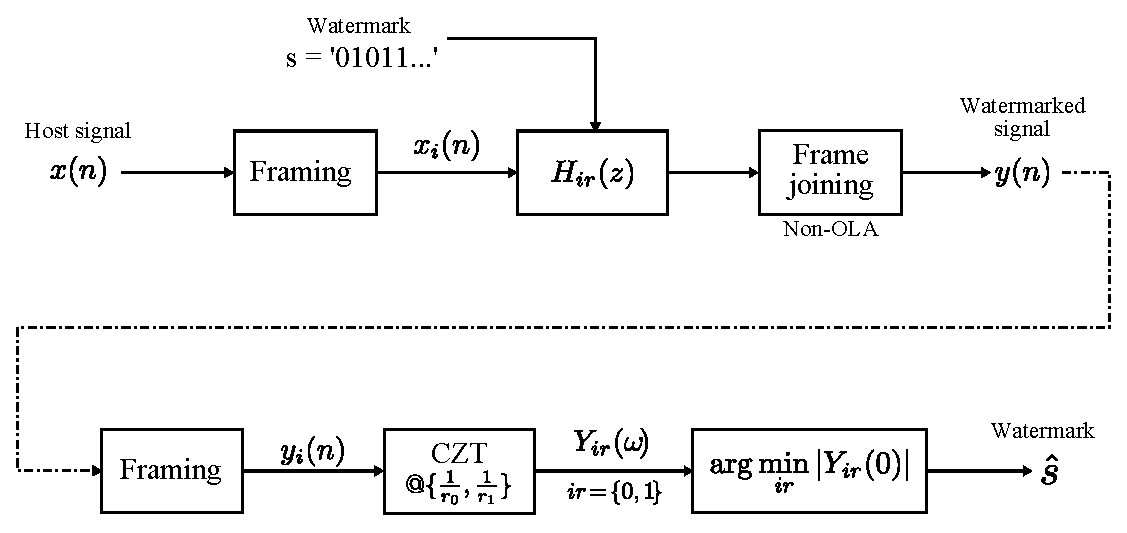
\includegraphics[width=1\textwidth]{PM_Scheme.eps}
  \caption{A scheme of audio data hiding based on phase coding: (a) watermark-embedding process and (b) watermark-detection process}
  \label{fig:pmscheme}
\end{figure}
The embedding process starts with frame segmentation of the host signal, \(x(n)\) into frames
\(x_i(n)\). Each watermark-bit from watermark \(s\) is embedded into one frame.

Figure \ref{fig:pmscheme} depicts a block diagram of the watermark-embedding process. A watermark-bit is em-
bedded into an audio frame as follows.
\begin{itemize}
\item{\textbf{Step 1.}} Original frame \(x_i(n)\) is transformed into the Fourier spectrum \(X_i(\omega)\) by FFT.
Magnitude spectrum \(|X_i(\omega)|\) and phase spectrum \(\angle X_i(\omega)\) are calculated.
\item{\textbf{Step 3.}} The watermark-bit are encoded into the phase of frequency-components by
QIM encoder and a quantized phase spectrum \(\angle Y_i(\omega)\) is obtained. Although each bit
can be embedded in only one component, it is embedded in all components to increase
robustness.
\item{\textbf{Step 3.}} The magnitude spectrum, \(|X_i(\omega)|\) and the quantized phase spectrum, \(\angle Y_i(\omega)\),
are combined into Fourier spectrum \(Y_i(\omega)\) and is then transformed into time domain signal
\(y_i(n)\) by inverse fast Fourier transform (IFFT).

\end{itemize}
Finally, all the processed frames are combined together to yield a watermarked signal
\(y(n)\).

\subsubsection*{Watermark detection}
The detection process also starts with frame segmentation of the watermarked signal,
\(y(n)\) into frames \(y_i(n)\). A Watermark-bit is detected from a watermarked frame as follows.

\begin{itemize}
\item{\textbf{Step 1.}} Watermarked frame \(y_i(n)\) is firstly transformed into \(Y_i(\omega)\) by FFT. Phase spectrum \(\angle Y_i(\omega)\)

\item{\textbf{Step 2.}} The phase of all frequency-components is decoded by QIM decoder all the bits. The output bit is determined by majority decision, e.g., if the number of `0' are greater the number of `1', the output is `0'.
\end{itemize}

These steps are repeated until we reach the final frame and all the watermark-bits are detected.
\section{Concurrency Programming}
\subsection{Basic concept}
Concurrency \cite{concurrency}is a concept comes from the field Communication Sequential Processes (CSP)\cite{csp}. In computer science, communicating sequential processes (CSP) is a formal language for describing patterns of interaction in concurrent systems. It is a member of the family of mathematical theories of concurrency known as process algebras, or process calculi, based on message passing via channels. 

Concurrency is the decomposability property of a program, algorithm, or problem into order-independent or partially-ordered components or units. This means that even if the concurrent units of the program, algorithm, or problem are executed out-of-order or in partial order, the final outcome will remain the same. This allows for parallel execution of the concurrent units, which can significantly improve overall speed of the execution in multi-processor and multi-core systems.

Large programs are often made up of many smaller sub-programs. For example, a web server handles requests made from web browsers and serves up HTML web pages in response. Each request is handled like a small program.

It would be ideal for programs like these to be able to run their smaller components at the same time (in the case of the web server to handle multiple requests). Making progress on more than one task simultaneously is known as concurrency. Go has rich support for concurrency using goroutines and channels.

\subsection{Golang}
Go\cite{golang} (often referred to as golang) is an open source programming language created by Google in 2007. It is a compiled, statically typed language in the tradition of Algol and C, with garbage collection, limited structural typing, memory safety features and CSP-style concurrent programming features added. The Go language has built-in facilities, as well as library support, for writing concurrent programs. Go introduces new concepts such as Goroutines and Channels to support concurrency programming. Those two are the basic blocks that made up our system.

\subsubsection*{Goroutines}
They're called goroutines because the existing terms—threads, coroutines, processes, and so on—convey inaccurate connotations. A goroutine has a simple model: it is a function executing concurrently with other goroutines in the same address space. It is lightweight, costing little more than the allocation of stack space. And the stacks start small, so they are cheap, and grow by allocating (and freeing) heap storage as required.

\subsubsection* {Channels}
Golang channels are pipelines to communicate between Goroutines. One Goroutine might has produced a value and want to send to other Goroutine, which would change behavior when receive this new value. This concept helps glue everything together and create a solid system of Goroutines working as a whole.

\begin{figure}
  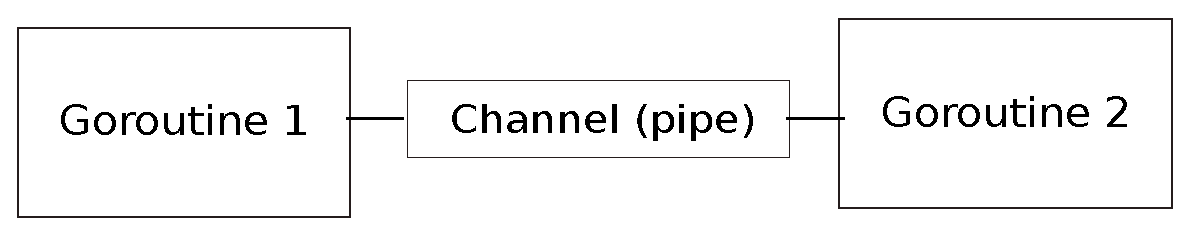
\includegraphics[width=1\textwidth]{goroutine.eps}
  \caption{Goroutines and channel}

\end{figure} % Background Theory 

\chapter{Audio Data Hiding based on Dynamic Phase Coding}
This section presents an audio data hiding method that we used in our project. This method implements the technique of embedding watermarks into the phase spectrum of audio signal. To increase robustness, we choose low frequencies regions to do embedding because most of audio information is stored at those ranges. This method of phase modification causes sound distortion in proportion with the magnitude of frequencies components. Hence, we base on the magnitudes to determine how much change we want to apply to the original phase components. By this, we can balance inaudibility and robustness. We also held experiments with our method and the results show that our watermarked audio signal is inaudible.
\section{Introduction}
Audio data hiding methods generally should satisfy following standards: \textit{inaudibility, blindness, robustness,} and \textit{high capacity}. There are many trade offs amongs these requirements that make it very hard to achieve a perfect solution. To maintain \textit{inaudibility}, we should employ watermark embedding at perceptually insensitive features. But on the other hand, audio processing can distort the watermark without degrading the audio quality. Therefore, it is a very important task in our embedding method that we choose the appropriate acoustic features that satisfy both \textit{inaudibility}, and \textit{robustness}.

In our embedding method, we divide audio data into frames and embed information directly into the samples in the time domain or frequencies components in the transformed domain. As we mentioned earlier, there are a lot of watermark embedding techniques. We focus on the phase coding method and employ the technique of QIM into the processing of frequencies components. Our experimental results show that the watermark is robust but the audio quality is decreased when the bit rate increases. We modify the phases of frequencies component based on how strong they are. The bigger the frequency magnitude, the less we apply QIM into the phase, in order to reduce sound distortion. In other words, the amount of phase modification is adjusted according to the frequency's magnitude. Strong frequency components are more sensitive to the amount of change in the phase of that component. Therefore, larger magnitude frequency components have small phase modification and vice versa. This is where we achieve both low sound distortion as well as robustness, which means a balanced trade off between \textit{inaudibility}, and \textit{robustness.} 

\section {Proposed Method}
\subsection{Quantization index modulation}
\begin{figure}[bt]
\center
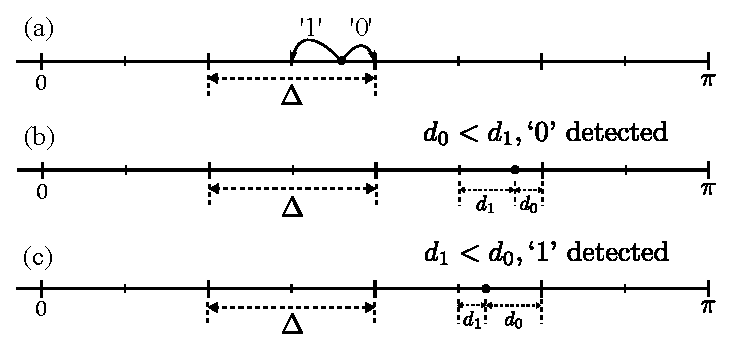
\includegraphics[width=.9\columnwidth]{QIMDemo_v1.eps}
\caption{Illustration of watermarking based on QIM: (a) embedding, (b) detection of `0', and (c) detection of `1'}
\label{fig:QIM}
\end{figure}
QIM has been considered as a class of provably good methods for digital watermarking \cite{qim}. The procedure of embedding and detecting watermarks is quite simple. Figure \ref{fig:QIM} shows an illustration of embedding and detection processes. To embed a bit $m$, `0' or `1' into a scalar variable $x$, we quantize $x$ to the nearest point that is an even or odd multiple of $\frac{\Delta}{2}$, respectively as (\ref{eq:QIMEncoder}). The obtained variable, $y$, is sent to receivers and might be affected by channel noise, hence becomes $\hat{y}$. To decode the embedded bit from $\hat{y}$, we calculate the distances between $\hat{y}$ and the nearest even multiple of $\frac{\Delta}{2}$, $d_0$ and the nearest odd multiple of $\frac{\Delta}{2}$, $d_1$ and then compare $d_0$ and $d_1$ to decode the bit as (\ref{eq:QIMDecoder1}) and (\ref{eq:QIMDecoder2}).

\label{eq:QIMEncoder}
\begin{align}
\label{eq:QIMEncoder}
y = Q(x,m) =
\begin{dcases} 
\Delta\left\lfloor\frac{x}{\Delta}+\frac{1}{2}\right\rfloor &\mbox{if } m = \mbox{`0'}\\ 
\Delta\left\lfloor\frac{x}{\Delta}\right\rfloor + \frac{\Delta}{2} &\mbox{if } m = \mbox{`1'}
\end{dcases}
\end{align}
where $\lfloor .\rfloor$ is the floor function and $\Delta$ is the QIM step size.
\begin{align}
\label{eq:QIMDecoder1}
d_j &= \hat{y} - Q(\hat{y},j), \quad j = \{\mbox{`0'},\mbox{`1'}\} \\
\label{eq:QIMDecoder2}
\hat{m} &= \arg\min_j d_j
\end{align}

\subsection {Principle of dynamic phase coding}
The original audio signal is processed by applying QIM to the phase spectrum. The result is a inaudible, robust, and reliable audio watermarking system with the following characteristics:
\begin{itemize}
\item{Phase modification is inaudible, that makes our embedded watermark is also inaudible}
\item{Most of audio information is distributed in low frequencies, thus this frequency region is more robust against attacks and should be chosen for embedding}
\item{Amount of change in the phase spectrum makes sound distortion in proportion with the magnitude spectrum of that frequency component. Therefore, we based on the magnitude to determine how much change we apply into the phase spectrum}
\item{Frequency components with extremely low magnitude are non-meaningful and very unreliable. So, we exclude those componens from our embedding process by establish a magnitude threshold.}

In the section, we investigate whether our method can help increase robustness while maintain the inaudibility by examine the above points.
\end{itemize}

\subsection{Watermark embedding}
We start off by spliting an original audio signal \(x(n)\) into many smaller frames \(x_i(n)\) with a fixed frame length. We also have a watermark string that is represented by binary bits \(s_i(l)\). We will employ the steps in Figure 4.2 to embedd \(s_i(l)\) into \(x_i(n)\).
\begin{itemize}
\item{\textbf{Step 1.}} Original frame \(x_i(n)\) is transformed into the Fourier spectrum \(X_i(\omega)\) by fast Fourier transform (FFT). Magnitude spectrum \(|X_i(\omega)|\) and phase spectrum \(\angle X_i(\omega)\)are calculated.
\item{\textbf{Step 2.}} We exclude the frequencies components whose magnitude are too small from the the embedding process. Specifically, we select the components whose magnitudes are larger than \(0.001\).

We then apply a dynamic phase coding system into our process. QIM step sizes are the amount of phase modification is determined based on its corresponding magnitude. First, magnitudes are normalize to 1 and linearly divided into \(L\) ranges in which each ranges has a corresponding step size. The higher the range, the smaller the step size.

Suppose that we have a set of \(L\) QIM step sizes, $\{\Delta_1, \Delta_2, ..., \Delta_L\}$, where $\Delta_1 > \Delta_2 > ... > \Delta_L$. The QIM step size for an embedding component $f$, namely $\Delta$, is determined as follows.

\begin{align}
%\nonumber |\hat{X}_i(f)| &= \frac{|X_i(f)|}{\max(|X_i(\omega)|)} \\
%\Delta &= \Delta_u, \mbox{where}\ u = \lceil L |\hat{X}_i(f)| \rceil
\nonumber |\hat{X}_i(f)| &= \frac{|X_i(f)|}{M} \\
\Delta &= \Delta_u,
\end{align}
 where $u = \lceil L |\hat{X}_i(f)| \rceil$ (if $u>L$, $u=L$) and $M$ is the parameter that represents for the maximum amplitude of most frequency components.

\item{\textbf{Step 3.}}  The bits $s_i(\ell)$ are encoded into the phase of the selected components by (\ref{eq:QIMEncoder}) and a quantized phase spectrum $\angle Y_i(\omega)$ is obtained. Although each bit can be embedded in only one component, it is embedded in several components to increase robustness. The bit rate is adjusted by changing the number of components for each bit.

\item{\textbf{Step 4.}} The magnitude spectrum, $|X_i(\omega)|$ and the quantized phase spectrum, $\angle Y_i(\omega)$, are combined into Fourier spectrum $Y_i(\omega)$ which is then transformed into time domain signal \(y_i(n)\) by inverse Fourier transform (IFFT).

Finally, all the processed frames are combined together to yield a watermarked signal \(y_n()\).

\end{itemize}

\begin{figure}[tp]
\center
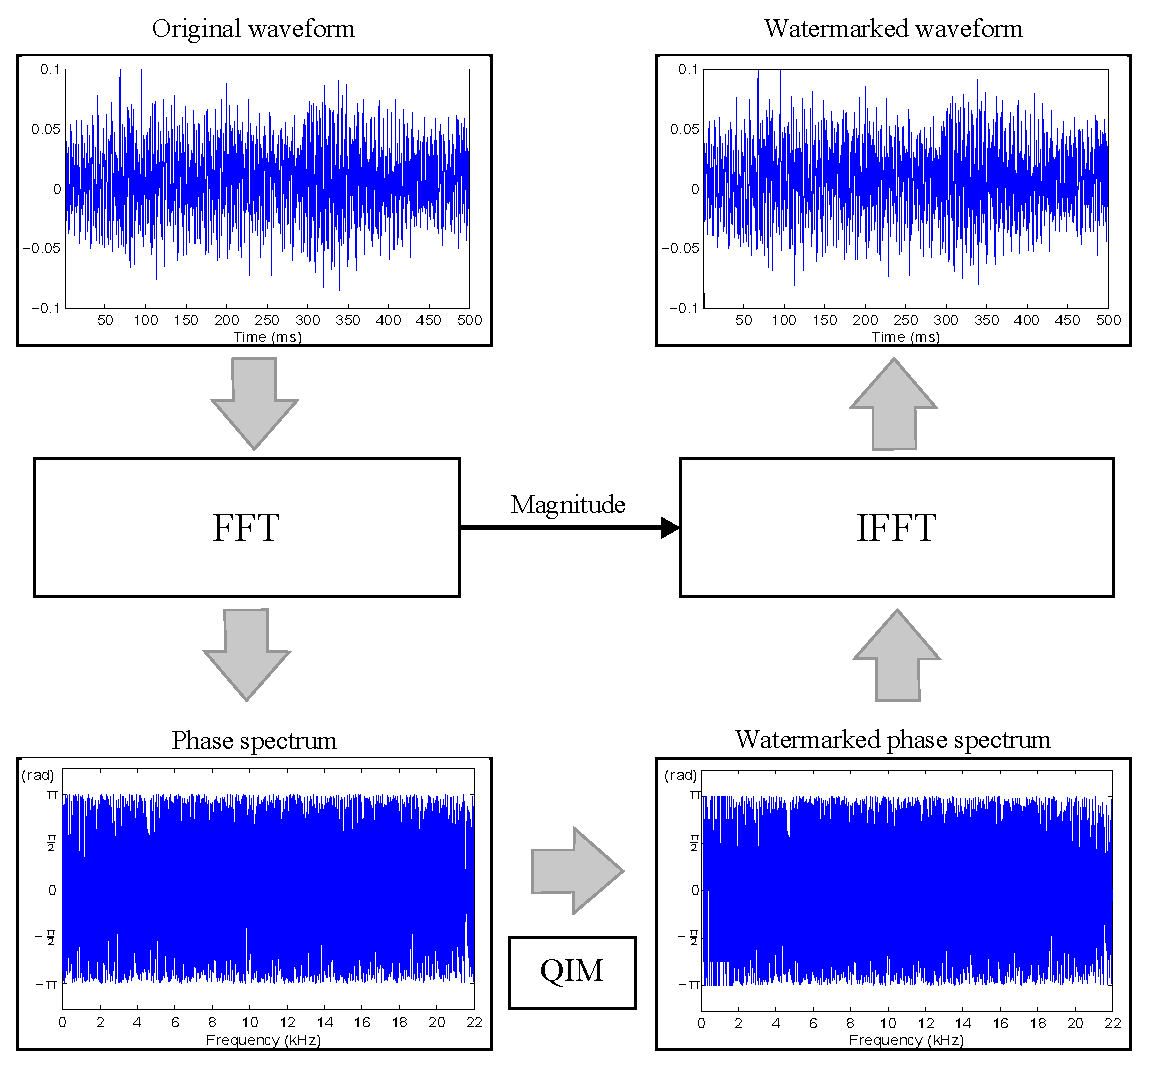
\includegraphics[width=1\columnwidth]{Illustrative_Example.eps}
\vspace{0mm}
\caption{Process of watermark embedding: conversion of a frame of time-domain samples into the Fourier domain, QIM watermark addition, and conversion back to the time-domain.
}
\label{fig:QIMWM_illustrative}
\vspace{0mm}
\end{figure}
\vspace{0mm}

% --------------------------------------------------------------------------

\begin{figure}[tp]
\center
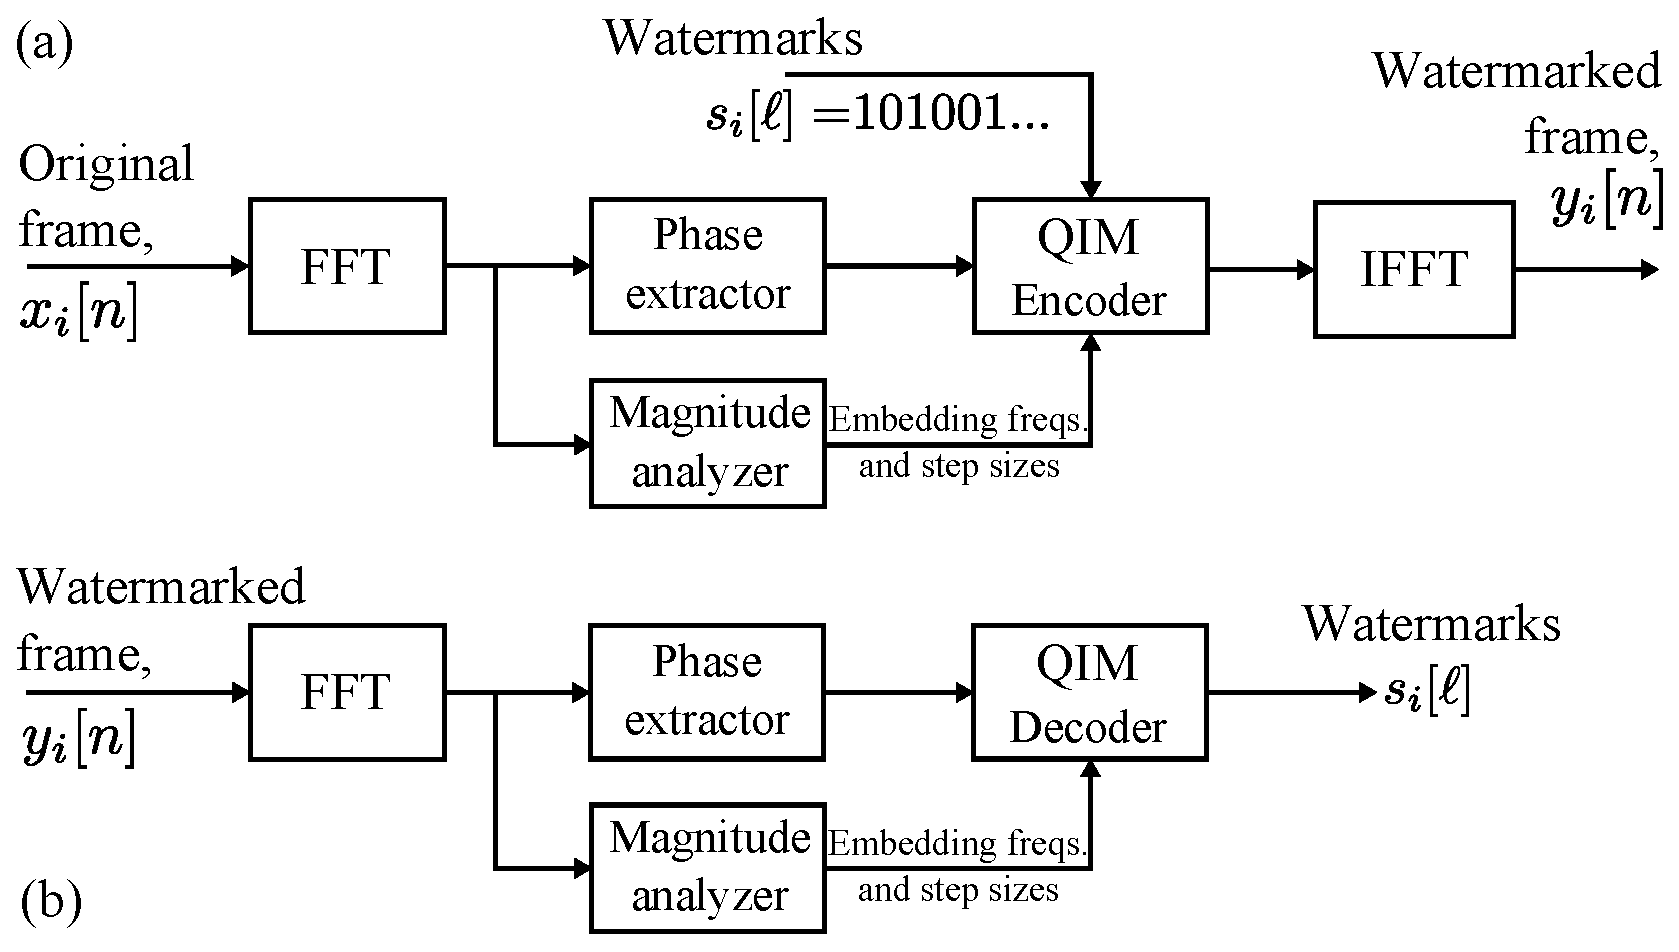
\includegraphics[width=1\columnwidth]{ProposedScheme.eps}
\caption{Proposed scheme of audio watermarking: (a) embedding process and (b) detection process}
\label{fig:WMScheme}
\end{figure}

\subsection{Watermark detection}
The detection process also starts with frame segmentation of the watermarked signal, \(y(n)\) into frames \(y_i(n)\) with the same frame size as in the embedding process. Figure \ref{fig:WMScheme}(b) shows a block diagram of the process that detects watermark bits from a watermarked frame involving three steps as follows.

\textbf{Step 1.} Watermarked frame \(y_i(n)\) is firstly transformed into $Y_i(\omega)$ by FFT. Phase spectrum $\angle Y_i(\omega)$ is calculated.

\textbf{Step 2.} The embedding frequency components and corresponding QIM step sizes are determined as in Step 2 in the embedding process.

\textbf{Step 3.} The embedding components are decoded by (\ref{eq:QIMDecoder2}) to extract all the bits. The output bits, $s_i(\ell)$, are determined by majority decision, e.g., if the number of `0', $N_0$, are greater the number of `1', $N_1$, the output is `0'.

These steps are repeated until we reach the final frame.
% -------------------------------------------------------------------------

\section{Evaluations}
\subsection{Parameters}
Before demonstrate our experiment, we would introduce many constant used in our entire project, including this experiment. Our system depends on many parameters in the process of watermark embedding. As we mentioned earlier, it is difficult to achieve an ideal settings when we have many dimensions. For instance, keeping the error rate low enough to not produce an incomplete watermarking, or else it would affect greatly on the user experience. At the same time, we also have to maintain a reasonable amount of embedding space to satisfy the embedding need. Those two are the biggest trade-offs of our system. It then becomes very important to experiement with different settings to come up with a optimal solution for our specific problem. There are two parameter that we need to keep eyes on.

\begin{table}
\centering
\caption{Configuration on the QIM step sizes with regard to the normalized magnitude}
\vspace{2mm}
\addtolength{\tabcolsep}{-6pt}
\begin{tabular}{|m{3cm}|m{2.25cm} | m{2.25cm} | m{2.25cm} | m{2.25cm} | m{2.25cm} m{0cm}|}
 \hline 
& \multicolumn{5}{c}{QIM step sizes ($\Delta$)} & \\ [.2cm]
\hline
Normalized magnitude & (0, 0.2] & (0.2, 0.4] & (0.4, 0.6] & (0.6, 0.8] & (0.8, 1] & \\
\hline
Set 1 & $\tfrac{\pi}{2}$ & $\frac{\pi}{4}$ & $\frac{\pi}{6}$ & $\frac{\pi}{8}$ & $\frac{\pi}{10}$ & \\ [.2cm]
\hline
Set 2 & $\tfrac{\pi}{3}$ & $\frac{\pi}{5}$ & $\frac{\pi}{7}$ & $\frac{\pi}{9}$ & $\frac{\pi}{11}$ & \\ [.2cm]
\hline
Set 3 & $\tfrac{\pi}{4}$ & $\frac{\pi}{6}$ & $\frac{\pi}{8}$ & $\frac{\pi}{10}$ & $\frac{\pi}{12}$ & \\ [.2cm]
\hline
\end{tabular}
\addtolength{\tabcolsep}{6pt}
\label{tab:QIMStep}
\end{table}

\subsubsection{QIM step sizes}First, as we employ the teachnique of dynamic phase coding, we depend on the magnitude of frequency coponents to determine the appropriate phase change. Specifically, we divide our frequency range into \(5\) small part, each with its own setting called step sizes. This number step size is very important to embedd into the phase component of the frequency. If we apply too much shift into the phase components, the audio quaility would decrease. Otherwise, too subtle change could not be successfully decoded. To figure out the best settings, we have to set up several experiments with different ranges of step sizes and record the resulting audio quality as well as the correctness percentage. The QIM step sizes are chosen as integer divisions of \(\pi\)
to reduce wrapping errors. We investigated the proposed method with three sets of five
QIM step sizes as shown in Table \ref{tab:QIMStep}.
\subsubsection{Embedding space}
We want to measure how many bits we have in 1 second for our watermark embedding to be effective while still satisfy acceptable capacity. In audio processing, we normally use a sampling frequency of \(44.1kHz\). Audio data is splitted into frames with a fixed frame length of \(22050\). While the audio data is stored in \(16\) bit integers. We have our sampling frequency equals \(44.1kHz\), which means there are \(44100\) integers of audio data in \(1\) second. Hence, if we choose our frame length equals \(22050\), each frame would be \(0.5\) second and bits per second is twice bits per frame \((BpS=2BpF)\). 

In the process of transforming audio data in time domain to the frequency domain, we can choose the range to apply the transformation. At this stage, we can either transform the whole audio file at once or split into smaller frames with fixed length. If we put the whole file into Fourier Transform at once, the frequencies along the files would be mixed together, produce an array of frequencies components from small to big frequency. Numerous components with the same frequencies would be merge into one as our transformation result. Clearly, this approach does not efficient in terms of computation and physics. On one hand, it adds memory overhead as we need to store the enormous transformation result the whole time, while we only need to store a much smaller amount if we split the file into frames. Moreover, mixing frequencies components into only \(1\) component and apply modification would result in the change in all the frequencies components corresponding to that frequency, and of couse this would harm both our audio quality and embedding correctness. Hence, we chose the second approach, spliting audio data into frames with fixed length. However, this result leads us to another question that, what is the resonable length for a frame? 
According to the Nyquist-Shannon sampling theorem, which states that, for a given sample rate \(f_s\), perfect reconstruction is guaranteed possible for a bandlimit \(B<\frac{f_s}{2}\). Plus, recall that the common maximum frequency that human ear can percept is approximately \(20kHz\). Which means, to effectively sample our audio data, we should choose the sample rate \(f_s>40kHz\). It is common in the field of audio processing that we choose \(f_s=44100Hz\) and frame length \(FL=\frac{f_s}{2}=22050\). 

In order to decrease the possibility of embedding into unstable frequencies components, which usually located at frequencies higher than \(1600Hz\). In fact, this low frequency region is where most of the sound content lies. Therefore, from the property of discrete Fourier transform, the bin corresponding to \(1600Hz\) frequency is at the \(\frac{FL}{f_s}1600=800^{th}\) bin. Hence, we only have \(800\) frequency bins to do embedding.

Next, we look closer into the \(800\) bins we got. To further increase our correctness, we repeat each bit consecutively many times. In particular, we chose \(BITREPEAT=5\), if we have \(1\) bit is incorrectly decoded, we still have \(4\) other bits to rely on. This greatly increase our embedding correctness. As we chose \(BITREPEAT=5\), we only have \(\frac{800}{5}=160\) bits left. But \(8\) bits form a character, which left us \(20\) characters per frame. 
\subsubsection{Summary}
In summary, we have the following parameters
\begin{itemize}
\item{\textbf{Step sizes}} We use 3 arrays of step sizes as described in Table \ref{tab:QIMStep}
\item{\textbf{Maximum number of embedding samples per frame}} \(SpF=800\)
\item{\textbf{Maximum number of embedding bits per frame}} \(BpF=160\)
\item{\textbf{Maximum number of embedding bits per second}} \(BpS=320\)
\item{\textbf{Maxium number of embedding characters per second}} Character per second \(CpS=40\)
\item{\textbf{Bit repeats}} Number of times repeat a bit to ensure embedding correctness \(BitRepeat=5\)
\item{\textbf{Minumum frequency magnitude for embedding}} \(MagnitudeThreshold=0.001\)
\end{itemize}
\subsection{Experiment metrics}
\subsubsection*{Audio quality}
Inaudibility is tested by PEAQ which rates sound quality by the ODG from −4 (very annoying) to 0 (imperceptible).
\subsubsection*{Embedding correctness}
Bit detection rate is measured by BDR, the ratio between the numbers of correct bits and total bits.

Character detection rate is measured by CDR, the ratio between the number of correct characters and total characters.
\subsection{Effectiveness of proposed method}
The result of our test is shown as below. Relate from \ref{tab:QIMStep}, because of bigger phase modification, the first setting show better perfomance in terms of BDR and CDR, which are both at 99.97\%. The details of result is shown in Table \ref{tab:bdrcdr}.
\begin{figure}
\begin{center}
\begin{tabular}{ |c|c|c| } 
 \hline
  			& BDR & CDR \\ 
 Settings 1 &  99.97\% & 99.97\% \\ 
 Settings 2 &  99.96\% & 99.92\% \\ 
 Settings 3 &  99.93\% & 99.87\% \\ 
 \hline
\end{tabular}
\end{center}
\caption{BDR and CDR test result}
\label{tab:bdrcdr}
\end{figure}

\begin{figure}[h]
	\centering
\includegraphics[width=\textwidth]{cdrmarkstream}
 	\caption{Character detection rate test result.}
 	\label{fig:CDRMarkstream}
\end{figure}

\section{Summary}
We proposed an audio watermarking method based on dynamic phase coding. Watermarks are embedded into low frequency components and the amount of change is determined based on the magnitude spectrum to balance inaudibility and robustness. We also employ 2 experiments to value the effectiveness of our proposed method. Our experiment had been carried to confirm the effectiveness of the DPC scheme.

The experimental results suggest that the proposed DPC scheme is more effective
than the SPC scheme, resulting in a better trade-off among the properties.
The proposed method is capable of embedding watermarks into audio signals at a
bit rate of 320 bits per second with the highest accuracy of watermark detection of 98\%. It has been re-vealed that the proposed method could satisfy the requirements of inaudibility, blindness, high capacity, and high reliability.  % Experimental Setup

\chapter{Proposed System}
\section{Overview}
Last chapter we discuss the audio data hiding method, which plays an important role in our system. It is the core that other parts of our system revolve around. However, without a logic system to flow data, the core has nothing to process and output. Recall that our project is about an streaming system that integrate watermark embedding before the streaming process. The output of our endpoint are audio data that are watermarked. Therefore, there are many processes that we need to take care, each will interact with each other to work together as a whole system.

Our system comprises of the server and client application. On the client side, we have 2 things to keep in mind: Audio watermark decoding and audio playback. Very straightforward, the audio data is decoded by a watermark decoding process and then sent to the playback component. If the audio fragment contains a embedded watermark, display the information when the sound is played. On the other hand, the server requires more considerations for its complexity. There are many things happening at 1 point of time on the server. While constantly waiting for the desired information to embed, we also do audio processing and produce audio data. That very audio data is sent to another module responsible for streaming to clients. Not to mention managing clients connection and authentication should not be taken lightly. Therefore, ideally, our server application contains smaller modules that independently contribute to the system as a whole, working together in harmony without stepping on each others toes. First, if an embedding information is received from the input, this module sends signal to the audio processing to do embedding. Afterwards, the audio module itself continues the flow by sending the embedded data to the streaming service and broadcast to clients. Moreover, all of those mentioned procedures independently execute on their own. For example, the streaming service continually sends data to clients and does not care if the data contains embedded information or not. 

We need an audio watermark process, obviously. This part takes audio data and a watermark string as input. It then employ the audio watermark embedding method we proposed last chapter and produce watermarked audio data as output. Our logic system help send data to this process and take its output to other processes. Hence, other processes as watermark input and streaming process is needed. The input process runs continuously and wait for watermark input, then it send the information to audio watermark process. After the watermarking process done embedding, it send watermarked audio data to the streaming process. The streaming process send audio data to clients and then wait for the next audio data to come. These processes run on its own, independently and send its result to other processes. Overall, we have a system illustrated in Figure \ref{fig:Server}. It’s also worth noting that we have our process running independently and interact with each other  to alter the flow of the program execution. In order to realize that, we need tools to employ such concept as concurrency. After identify the needed features of our server application, we realize that we need a framework to build those small modules and glue them together. To realize this idea, we came up with a system design that rely on the field of communicating sequential processes. Specifically, concurrency is our goal. Concurrency is a way to divide the existing big problem into smaller parts that are independent. This is where we take advantage of Golang and its support for concurrency.

\subsection{Server setup}

Seeing how complex the idea of concurrency is, we shift to finding a mechanism to realize this without implement it ourselves. Apparently, it is best that we apply the assistance from a specialized programing language. Partly, to accomplish our original idea, system designing is put at the highest priority, but it would be so much easier if we utilize on a programming language and its intrinsic properties that help us implement this more effectively. After much discussion, we bring another result of our research engineering process into the project as we choose Golang as the programming language for the server application. Golang is a relatively new programming language invented by Google with focus on concurrency. Golang features built-in properties that support concurrency. As mentioned earlier, we modularize our system into smaller parts that work independently. At this point, we apply the goroutine concept from golang to help achieve this. Goroutines are lightweight threads allocated for an instance of a function to execute independently. In our case, we have 4 goroutines that continually running. Golang also introduces channel, as a mean for goroutines to signal each other. For instance, if the input goroutine receive an actual input, it sends the input data through the channel that connects to the audio processing goroutine. Consequently, this function changes its way of processing audio data, switching to do audio embedding with the input data received. Otherwise, the audio processing module would only extract audio data, no watermarking is involed. The streaming goroutine does not care how the audio process deals with data, it only takes audio data that the audio module sends through a channel, and stream to clients. Meanwhile, if there are any new client connect to the streaming point, the client manager goroutine persist the connection for further data streaming. All of those goroutines works independently and signal each other for data. We call this share memory by communicating, not communicate by sharing memory. This is the main compass of the Golang programming language.

\begin{figure}[bt]
\center
\includegraphics[width=.9\columnwidth]{system.eps}
\caption{Our server flow chart}
\label{fig:Server}
\end{figure}

With the strong support from Golang, it becomes less painful when implementing the design architecture. However, what Golang does is simply provide us a tool to better systemizing. It is important that we have a solid ground of system design that Golang can relies on and do what it is best at. At the front line, we have the audio processing sequentially scans through the audio file and extract a frame of audio samples with fixed length. This frame is pushed into the queue waiting to be sent to the steaming module, where we also have a queue. The reason why we apply queues to handle data is congestion preventation while also assure a decent amount of spare space for unusually long watermarking information. Specifically, when a big input is received and the current audio frame is not enough for embedding, we should not wait for the next frame because it would increase the overhead cost for the system. What best is take the remaining frames in the queue and fill them up with embedding information. On the other hand, the streaming module also needs a queue to make sure the situation of data starve will not occur. Otherwise, without a queue, if the audio embedding takes too much time to complete, the client have to wait for data to produce sound to listeners, and that is not good at all.

\subsection{Client setup}
At the client, we would like to keep it as simple as possible, since this is where the user experience our product and it's wise to keep the implementation straightforward and less error prone. Therefore, we decided to choose the simple popular frontend web framework AngularJS\cite{angular}. This piece of technology require very little effort to get up and running. However, we still face some engineering obstacles. First, it is very important what technology we choose to establish a connection betweeen the server and client. We would like it to be a stream of continuous data, without having to re-create the connection each time new data is to be sent. There are many solution for our streaming, we can rely on a third party program like Gstreamer\cite{gstreamer} to do the streaming for us, or utilize a builtin feature of our very mechanism of connect to the internet: browser. 

We then do a small research and sketch out some strengths and weakness of the two ways. For Gstreamer, it would lift a burden for us doing streaming on it own, we only need to feed data for it and everything is set. Unfortunately, there is a high chance we can not integrate it into our existing system. Since streaming involves both the server and client and it less likely to combine many technologies together. On the other hand, if we invest resources into researching an intrinsic streaming feature of our existing system, which are Golang and AngularJS, we then can be sure about compatibility of our system. Afterward, we proceed to look for a suitable means for our streaming process. We found out that both Golang and AngularJs support websocket. Moreover, it is also a simple solution that we can pickup very quickly.

In the end, we have a client set up illustrated in Figure \ref{fig:Client}

\begin{figure}[bt]
\center
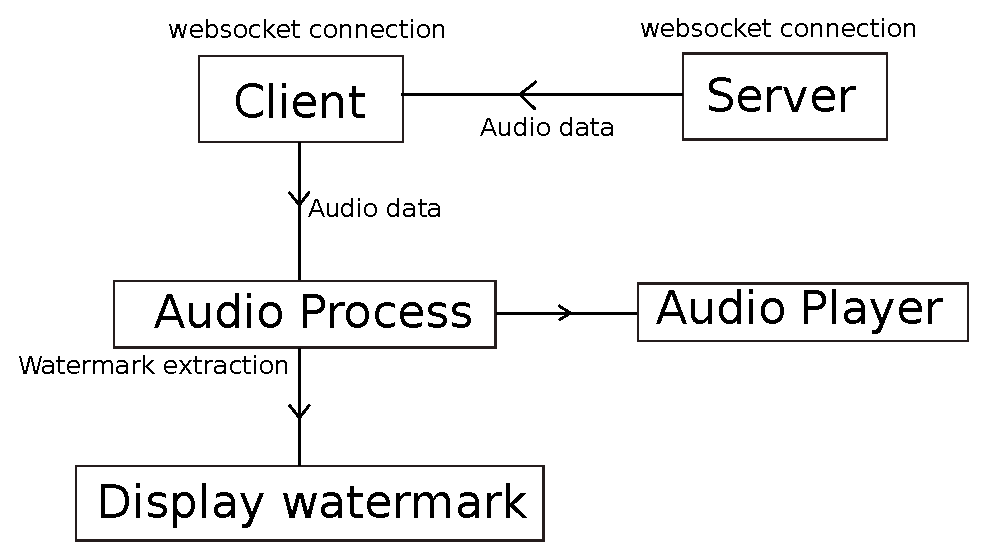
\includegraphics[width=.9\columnwidth]{client.eps}
\caption{Our client flow chart}
\label{fig:Client}
\end{figure}

\section{Proposed System in Details}
\subsection{Watermark Input Process}
Watermark input process is the first stone of our system, it acts as a receiver, waiting for input and send to other processes. Specifically, we spawn a Goroutine to execute on its own. When watermark is received, this process takes in characters as input and feed to a predefined channel. This channel associates with other processes and send watermark input to them. The input process is briefly illustrated in Fig \ref{fig:InputProcess}.

We would like the process to sleep for 5 seconds to avoid input abuse. Otherwise, if there are too many watermark strings to embed, it would be difficult to track result. We recommend that we put all our watermark strings into a big string to do embedding for only once.

\begin{lstlisting}
// Watermark Input Process
func (ms *MarkStream) Input() {
	reader := bufio.NewReader(os.Stdin)
	for {
		log.Printf("Input your embedding string: ")
		text, _ := reader.ReadString('\n')
		ms.userInputChan <- text
		log.Println("Embedding...")
		time.Sleep(5 * time.Second)
	}
}
\end{lstlisting}

\begin{figure}[bt]
\center
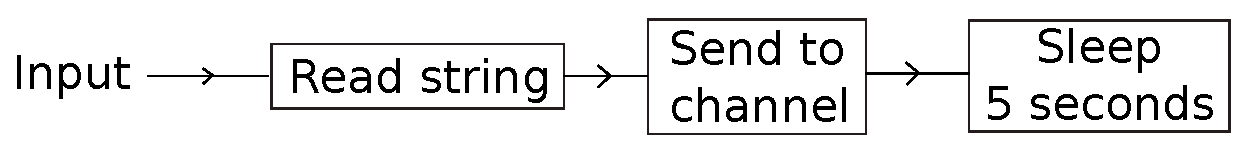
\includegraphics[width=.9\columnwidth]{inputprocess.eps}
\caption{Watermark receiver}
\label{fig:InputProcess}
\end{figure}

\subsection{Audio Watermarking Process}
\begin{figure}[bt]
\center
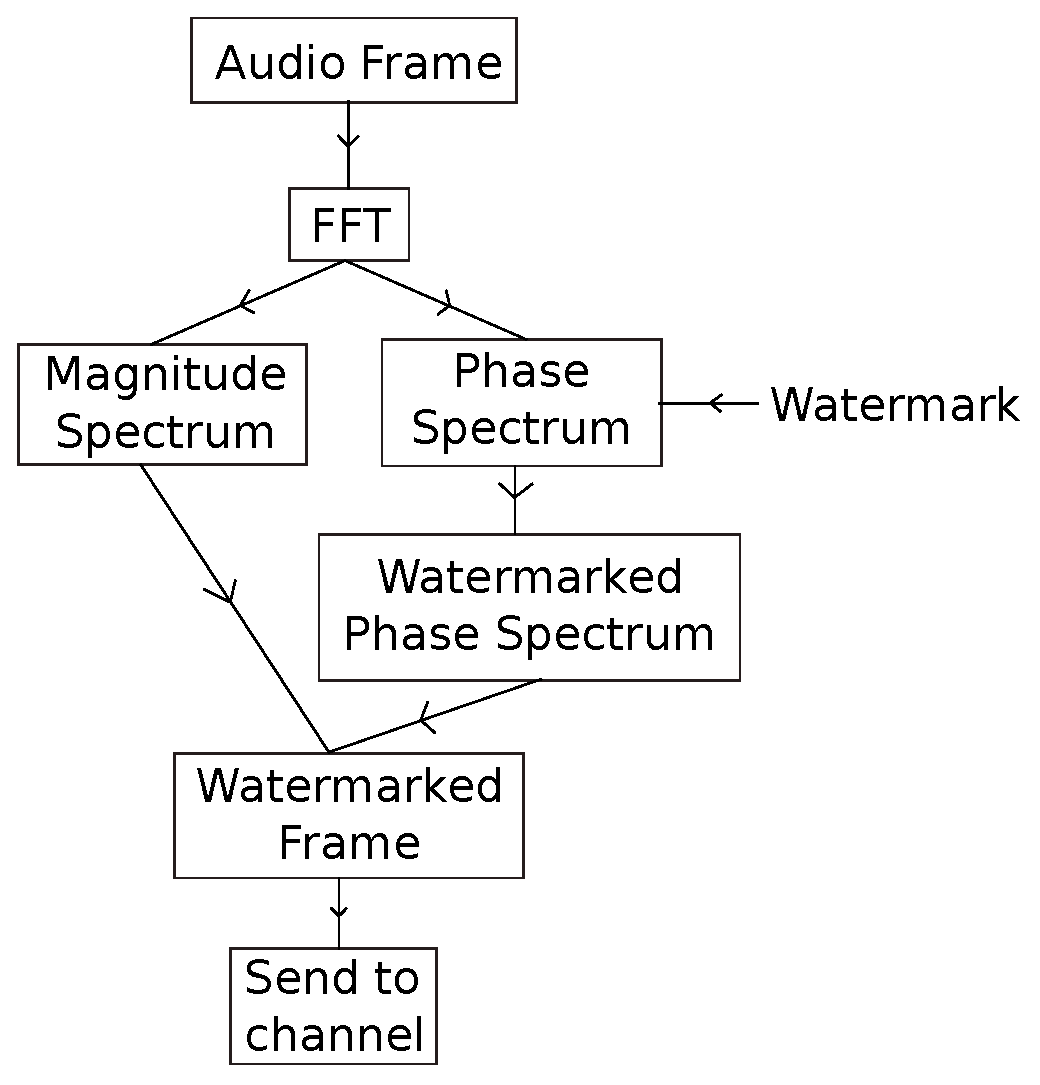
\includegraphics[width=.9\columnwidth]{watermarkingprocess.eps}
\caption{Audio watermarking process}
\label{fig:WatermarkingProcess}
\end{figure}
The core of our system lies at the audio watermarking processing. It should be noted that producing a good quality, low error rate, embedded audio file is not something could be taken by granted. Instead, it is a process of trade-offs that we must examine carefully. At the time of this research, there are many watermarking methods available. Some methods remove the least significant bits to make space for the watermark (LSB), or shape the watermark according to the human auditory system (HAS). Other methods use the simultaneous masking characteristics of HAS or relative insensitivity of phase change to embed inaudible watermarks. Phase coding is used because since controlled phase alteration results in inaudible change in sound to HAS. On the other hand, to improve robustness, quantization index modulation (QIM) is employed and has shown promising results with several audio watermarking methods. We would like to combine the greate result of inaudibility and robustness together to produce audio that not only has good quality but also solid against several attacks in robustness. The idea is to transform the original time domain audio data into frequency domain by Fourier transform (FFT is used). Result of the transformation is the magnitude and phase components of the frequencies bins. QIM is used here to embedd a bit, either 0 or 1, into the original phase. Depends on the magnitude component of the bin, we decide how much change we apply to the phase component. The result is new phase components that are slightly different compared to the original ones. Finally, using the Inverse Fourier tranform, we remake the audio data by combining the magnitude components and the new phase components. The final outcome is new audio data that are embedded. This method is called dynamic phase coding. It takes one step further than the tradition phase coding, where we only use one fixed amount of modification to adjust the phase. Since the audio features contains a lot of different frequencies, using just one standard can not cover all the possible values and end up only effective for a certain range of frequencies. Other ranges would result in either bad quality audio or highly error prone watermarking. 

Audio watermarking is the primary part of our system. It process audio data while also wait for watermark input and do embedding. If there is no input is received, ordinary audio data is produced. All of those output is sent to the streaming Goroutine to handle.

It’s important to know that audio file is made of mere integers, which is called samples. For our project, we represent an integer by 16 bits \(=2\) bytes. This process continuously waits for audio data to come  and perform necessary actions to do audio processing. Specifically, for each 500ms, it receives a slice of the data of length 22050 samples, which means \(22050*2=44100=44.1kB\). For the sake of our project development, we simply create another Goroutine responsible for sending out audio data. In reality, we would have a stream of audio of our own. The audio watermarking process is illustrated in \ref{fig:WatermarkingProcess}

Recall that the output of our server is a stream of audio data, nothing else. Therefore, there is a technical challenge about how to notify client when a watermark is embedded. We studied that the cost of audio embedding is not too much and we can do it without any overhead burden in terms of memory assumption and execution time. In fact, embedding an audio frame with framelength of \(22050\) only costs us \(0.05\) second. Therefore, we decided to embedd a notifying character to solve the problem of watermarking synchronization. There are two cases of flow control for this process.
\subsubsection*{There is no input received}
In this case, our embedding string is only a chacter \('0'\), which costs us \(8*5=40\) samples to embed, where 8 is the number of bits for character \('0'\) and 5 is how many times we repeat 1 bit to ensure embedding correctness. Then, when the client receive our audio data, they will employ watermark extraction and understand that there are no input embedded in this particular audio frame.
\subsubsection*{There is input received from the channel of the input process}
In this case, our embedding string is \('1' + input\). The steps of execution are the same and produce a watermarked audio frame. If the input to embed is too long and exceed the length of maximum samples we can embedd, which is \(800\), then we continue the embedding in the next audio frame. It's very crucial that we only do audio processing on the first \(800\) samples of the audio frame. Otherwise, we probably produce a low quality audio data and hightly error prone for watermark extraction.

\subsection{Client Managers and Audio Streaming Process}
We also have a client manager to store client's connections for streaming purpose. In engineering terms, we open a websocket endpoint waiting for clients to connect. Each time a client comes in, we spawn a temporary Goroutine reponsible for that particular client. In this specific Goroutine, we create a unique identity for this new client and save its connection in an array for further use. Then, this Goroutine ends asynchronously, only the array of client connection is preserved.

In this process, when we receive audio frame from the watermark embedding process, we iterate through the list of clients and send audio data to them. Another note is about the format for streaming over the Internet. The result of the watermarking process is an array of \(float64\) numbers. If we choose to broadcast this type of data over the Internet, the cost would be huge and potentially cause incompleted data. Therefore, we scale down the output to only \(int16\) type, which does not affect the accuracy of data much. By this way, we broadcast our audio data over the Internet with a minmized cost while still ensure its quality.

The technolgy we use to streaming is websocket\cite{websocket}. WebSocket is a protocol providing full-duplex communication channels over a single TCP connection. It is designed to be implemented in web browsers and web servers, but it can be used by any client or server application. The WebSocket Protocol is an independent TCP-based protocol. Its only relationship to HTTP is that its handshake is interpreted by HTTP servers as an Upgrade request. The WebSocket protocol makes more interaction between a browser and a web server possible, facilitating the real-time data transfer from and to the server. This is made possible by providing a standardized way for the server to send content to the browser without being solicited by the client, and allowing for messages to be passed back and forth while keeping the connection open. In this way, a two-way (bi-directional) ongoing conversation can take place between a browser and the server

\begin{lstlisting}
\\ Client Manager and Audio Streaming
func (ms *MarkStream) StreamServer(ws websocket.Connection) {
	cl := new(Client)
	cl.uuid = uuid.NewV4().String()
	cl.conn = ws
	ms.connManager.AddClient(cl)
}

func (m *Manager) StreamToClients() {
	for {
		select {
		case audioData := <-m.audioDataChan:
			for _, cl := range m.clients {
				err := cl.conn.EmitMessage(Int16ArrayByte(audioData))
				if err != nil {
					m.DeleteClient(cl.uuid)
				}
			}
		}
	}
}
\end{lstlisting}

\section{System Evaluation}
\subsection{Experiment context}
We list some quantities to measure the efficiency of our system in the context of the original objective of this thesis. In term of audio processing, we did provide some parameters and metrics to measure audio quality and embedding correctness in the last chapter. However, in this chapter we would like to understand how our system affect the way people conceive advertisements in Internet radio broadcasting. Therefore, we aim to create a simulation to test the real value of our system.

We capture real advertisement to do a simulation and present to actual user to compare the two version of advertisement: The normal advertisement and the augmented advertisement.
\subsection{Experiment settings}
It's very important that we set the environment of our simulation to resemble the traditional avertisement, so that the user can interact naturally with our system and produce reliable experiment result.

We record an advertisement from the popular Internet radio broadcasting service - Spotify\cite{spotify}, to use in our experiment. To correctly measure the effeciency of our advertising system, we focus on the number of user engagements compare with the normal system. With the normal advertisement, 12\% of listerners shown interests but only a few went further to look for extra information. On the onther hand, with our augemnted advertisements, listeners do not have to make that extra effort and therefore can jump right to the advertisement intention. 80\% of the listeners who shown interests appreciated the extra information that we deliver through watermarking. The experiment result exhibited that our advertisement system enhance the marketing efficiecy with augmented advertisements.

\section{Summary}
In this chapter, we propose a system of small processes rendered by Goroutines, in order to apply audio watermarking in Internet radio broadcasting. Our proposed system comprises of many small parts cooperating with each other and working as a whole. They work independently and communicate by channels, another builtin feature of our primary programming language - Golang. The result is a tight system that is not only coherent and produce no bugs but also very easy to comprehend for human. In terms of engineering, we have accomplished a goal set in the beginning of the thesis. We would like to create an integration of audio watermarking and Internet radio broadcasting.

On the other hand, another goal that we set for this thesis is about enhancing advertising efficiency by augmenting it with additional information. We had carried experiments to compare our system with traditional advertising method. The results have shown that our system has affects on the advertising efficiency of Internet radio broadcasting, where users engagements alot more than the traditional advertising method. % Experiment 1

\chapter{Conclusion}
\section{Summary}
Digital audio processing is a very large field that has a lot of application in the real world. After taking research in this area, we see the potential of its smaller branch: Audio data hiding, whose value not only about securing data but also enriching user experience in audio experiencing. In addition with the fact that our current method of audio advertising is poor in performance and lack user interaction, we aim to create a new advertising methodology combining audio watermarking and Internet radio broadcasting. While traditional audio advertisting focus only on the audio content to attract customers, we propose an extra gate of information for user to learn more about our advertisements. 

The result of our engineering project is a stable, standalone system that take audio data as input. In reality, our input may comes from an actual radio broadcasting station. We then employ the technique of audio data hiding to embedd extra advertising information to the audio data itself, producing a stream of watermarked audio data and stream to clients. On the other hand, the client application receive audio data, extract watermark and display to users, assisting them connect to our advertisments. 

We also conduct several experiments to validate our proposed methods in audio data hiding and an audio streaming system. The outcome of our experiments shown potential in applying a new method of advertising in Internet radio broadcasting.

\section{Contribution}
In this thesis project, we had contributed to Internet radio broadcasting and software engineering field the following points:
\begin{itemize}
\item{} We created a audio streaming system with audio data hiding integrated. This help validate the idea of enhancing user experience with augmented audio content. From that vantage point, there would be more doors to be opened in this Interet radio broadcasting industry. Moreover, this project can be a ground stone for future projects that are based on the idea of a audio streaming service combines with audio watermarking.
\item{} By employ the audio data hiding method of dynamic phase coding, we validate it again with convincing experiment results. Plus, we illustrate a correct implementation of this algorithm for future project to reference to.
\item{} With the use of Golang and its support for concurrency, we emphasize on a way of software engineering by dividing our system into independent parts operating on its own while also contribute to the system as a whole.
\end{itemize}

\section{Future Work}
There are alot of upgrade we would like to apply to this project. For instance, it is our initial intention that we apply the standard streaming protocol to this project, so that it would work everywhere, while we only need to provide a plugin client to extract and display watermark. Plus, the complexity of client application needs to be minimized, we should realize that by compress our project into a stable, compact black box or library. It would be easier to distribute and popularize our advertising method.

In terms of compatibility, our project operate on the WAV audio files, whose size is much larger than the compressed file type MP3. It would be better that we support input as other audio file types. However, as the goal of our project is to provide a system of audio streaming, regardless of input type. Because, ultimately, our input is an array of audio data, which is the result of MP3 decompression. Therefore, the problem of file types does not matter much in the future.

At the core of our project, we also need to upgrade the audio watermarking method too. It appears in the project that there are many settings of parameters, environments that we did not experiment with. For example, we limit ourselves with only 5 QIM step sizes. We believe that there are potential to upgrade our embedding method in terms of either embedding space or embedding correctness.

However, in business terms, it is more important that we first validate this project objective in a larger scale. While this thesis has shown some effects in enhancing user engagement in advertising, it is still unsure that the Internet radio broadcasting community would adapt our method and replace their existing technology.

In summary, we propose some issues that worth a reconsideration in the future as below:
\begin{itemize}
\item{In order to enhance the quality of audio watermarking, we can apply the new interesting field of machine leanring. By modeling the sound pattern of those which are easy to watermark and those which are error prone, we actually minimize the possibility of watermarking incorrectly.}
\item{Another possible way of upgrading the audio watermarking algorithm is experiment with various settings that we did not try in our project.}
\item{We should apply the industry standard mechanism of streaming.}
\item{Minimize the complexity of client application to make it easier to distribute and install. Allow the community to adapt to our method.}
\item{A mechanism for listener to interactively respond to advertisements. At the moment, it is just pure audio playback that are less likely to attract customer to the advertiser's intention. Not only providing a means for richer static content such as text, images, we aim to put in dynamic functionalities that take input from user. From that, analyze those inputs and take a further step in understanding customer and delivering more relevant advertisement.}
\end{itemize} % Experiment 2

%\input{Chapters/Chapter6} % Results and Discussion

%\input{Chapters/Chapter7} % Conclusion

\begin{thebibliography}{9}
\bibitem{edison2016} 
Infinite Dial report from Edison Research.
\\\texttt{http://www.edisonresearch.com/the-infinite-dial-2016/-}
[Online, accessed 20-July-2016]

\bibitem{edisonslide} 
Infinite Dial slides report from Edison Research.
\\\texttt{http://www.slideshare.net/webby2001/infinite-dial-2016}
[Online, accessed 20-July-2016]

\bibitem{xapp2015q1} 
Xapp Media Internet radio ad load report Q1 2015.
\\\texttt{http://xappmedia.com/wp-content/uploads/2015/01/Internet\-{}Radio\-{}Trends-Report\-{}2015\_{}january.pdf}
[Online, accessed 20-July-2016]

\bibitem{xapp2015q4} 
Xapp Media Internet radio ad load report Q4 2015.
\\\texttt{https://xappmedia.com/download-internet-radio-ad-load-report-2015/}
[Online, accessed 20-July-2016]

\bibitem{spotify} 
Spotify
\\\texttt{https://www.spotify.com}
[Online, accessed 20-July-2016]

\bibitem{peaq} 
PEAQ Standard
\\\texttt{https://en.wikipedia.org/wiki/PEAQ}
[Online, accessed 20-July-2016]

\bibitem{has} 
Human Audiotory System
\\\texttt{https://en.wikipedia.org/wiki/Auditory\_{}system}
[Online, accessed 20-July-2016]

\bibitem{qim} 
Quantization Index Modulation
\\\texttt{http://allegro.mit.edu/pubs/posted/journal/2001\-{}chen\-{}wornell\-{}jvlsi.pdf}

\bibitem{echohiding}
D. Gruhl, A. Lu, and W. Bender, “Echo hiding,” in Proc. of Information Hiding,
LNCS 1174, pp. 295–315, 1996.
[\textit{On the electrodynamics of moving bodies}]. 
Annalen der Physik, 322(10):891–921, 1905.
 
\bibitem{moore} 
B. C. J. Moore, \textit{An Introduction to the Psychology of Hearing 6th ed}. Brill Academic
Pub, 2013.

\bibitem{ozawa} 
K. Ozawa, Y. Suzuki, and T. Sone, \textit{Monaural phase effect on timbre of two signals}, Journal of Acoustic Society American, vol. 93, no. 2, pp. 1007–1011, 1993.

\bibitem{mp3} 
MP3 audio encoder [Online, accesed on \(20^{th}\) July, 2016]
\\\texttt{https://en.wikipedia.org/wiki/MP3}

\bibitem{aiba} 
E. Aiba, M. Tsuzaki, S. Tanaka, and M. Unoki, \textit{Judgment of perceptual synchrony
between two pulses and verification of its relation to cochlear delay by an auditory
model}, Japanese Psychological Research, vol. 50, no. 4, pp. 204–213, 2008.

\bibitem{yasi} 
J. A. Yasi, \textit{An algorithm for extracting the relative phase of harmonics from a peri-odic digital signal.}
\\\texttt{http://physics.illinois.edu/undergrad/reu/2004/Yasi.
pdf, 2004}

\bibitem{yost} 
W. A. Yost, A. N. Popper, and R. R. Fay, \textit{Auditory perception of sound sources}, Springer, 2008.

\bibitem{dong} 
X. Dong, M. F. Bocko, and Z. Ignjatovic, \textit{Data hiding via phase manipulation
of audio signals}, in Proc. of International Conference on Acoustics, Speech, and
Signal Processing, vol. 5, pp. 377–380, 2004.

\bibitem{concurrency} 
Concurrency
\\\texttt{https://en.wikipedia.org/wiki/Concurrency\_{}(computer\_{}science)}

\bibitem{csp} 
Communicating sequential processes
\\\texttt{https://en.wikipedia.org/wiki/Communicating\_{}sequential\_{}processes}

\bibitem{golang} 
Golang
\\\texttt{https://golang.org}

\bibitem{gstreamer} 
Gstreamer
\\\texttt{https://gstreamer.freedesktop.org/}

\bibitem{angular} 
AngularJS
\\\texttt{https://angularjs.org/}

\bibitem{websocket} 
WebSocket
\\\texttt{https://en.wikipedia.org/wiki/WebSocket}

\bibitem{fft} 
The Fourier Transform
\\\texttt{http://www.thefouriertransform.com/}

\bibitem{tritonreport} 
Triton March 2016 Webcast Metrics Top 20 Ranker
\\\texttt{https://xappmedia.com/triton-data-shows-continued-rise-internet-radio-listening/}

\bibitem{edisonresearch} 
The Infinite Dial report from Edison Research and Triton Digital
\\\texttt{https://xappmedia.com/edison-research-internet-radio-weekly-listeners-half-us-population/}

\bibitem{nmnhut} 
N. M. Ngo, M. Unoki, R. Miyauchi, and Y. Suzuki, \textit{Data hiding scheme for ampli-
tude modulation radio broadcasting systems,}, Journal of Information Hiding and
Multimedia Signal Processing, Ubiquitous International, vol. 5, no. 3, pp. 324–341,
2014.

\bibitem{nmnhutpaper} 
Nhut Minh Ngo, Brian Michael Kurkoski, and Masashi Unoki, \textit{ROBUST AND RELIABLE AUDIO WATERMARKING BASED ON
DYNAMIC PHASE CODING AND ERROR CONTROL CODING}, 23rd European Signal Processing Conference (EUSIPCO) 
\\\texttt{http://www.eurasip.org/Proceedings/Eusipco/Eusipco2015/papers/1570104339.pdf}

\bibitem{dwalliance} 
DIGITAL WATERMARKING PLAYS EXCITING ROLE IN ENHANCING ENTERTAINMENT EXPERIENCES FOR CONSUMERS THROUGH TELEVISION, MAGAZINES AND MOBILE DEVICES
\\\texttt{http://www.digitalwatermarkingalliance.org/pr\_{}10JUL2012.asp}

\end{thebibliography}

%% ----------------------------------------------------------------
% Now begin the Appendices, including them as separate files

\addtocontents{toc}{\vspace{2em}} % Add a gap in the Contents, for aesthetics

\appendix % Cue to tell LaTeX that the following 'chapters' are Appendices

\chapter{Appendix}

\section{Source Code}
\subsection{Audio Watermarking Process}
\begin{lstlisting}
// Audio Watermarking Process
func (ms *MarkStream) Embedding(l []float64) {
	var i = SAMPLE_PER_FRAME - 1
	var j = 0

	for i < len(l) {
		select {
		case watermark := <-ms.userInputChan:
			var pos = 0
			submag := make([]float64, i+1-j)
			subphs := make([]float64, i+1-j)
			var stringbit = PrepareString("1" + watermark + "\n")
			for pos < len(stringbit) {
				var subl = l[j : i+1]
				subfourier := fft.FFTReal64(subl)
				var count = 0
				var bitrepeat = 0

				for k, x := range subfourier {
					submag[k], subphs[k] = cmplx.Polar(x)
					if submag[k] < MAG_THRES {
						continue
					}
					if pos < len(stringbit) && count < BIN_PER_FRAME {
						subphs[k] = QIMEncode(submag[k], subphs[k], int(stringbit[pos]))
						count++
						bitrepeat++
					}
					if bitrepeat == BIT_REPEAT {
						bitrepeat = 0
						pos++
					}
				}

				cmplxArray := make([]complex128, len(subl))
				for i, _ := range cmplxArray {
					cmplxArray[i] = cmplx.Rect(submag[i], subphs[i])
				}
				newWav := fft.IFFTRealOutput(cmplxArray)
				Wav16bit := Scale(newWav)
				ms.connManager.audioDataChan <- Wav16bit
				j = i + 1
				i += SAMPLE_PER_FRAME
				if len(l)-i > 0 && len(l)-i < SAMPLE_PER_FRAME {
					i = len(l) - 1
				}
				time.Sleep(400 * time.Millisecond)
			}
		default:
			var pos = 0
			var subl = l[j : i+1]
			subfourier := fft.FFTReal64(subl)
			submag := make([]float64, i+1-j)
			subphs := make([]float64, i+1-j)
			var stringbit = PrepareString("0")
			for pos < len(stringbit) {
				var count = 0
				var bitrepeat = 0

				for k, x := range subfourier {
					submag[k], subphs[k] = cmplx.Polar(x)
					if submag[k] < MAG_THRES {
						continue
					}
					if pos < len(stringbit) && count < BIN_PER_FRAME {
						subphs[k] = QIMEncode(submag[k], subphs[k], int(stringbit[pos]))
						count++
						bitrepeat++
					}
					if bitrepeat == BIT_REPEAT {
						bitrepeat = 0
						pos++
					}
				}

			}
			cmplxArray := make([]complex128, len(subl))
			for i, _ := range cmplxArray {
				cmplxArray[i] = cmplx.Rect(submag[i], subphs[i])
			}
			newWav := fft.IFFTRealOutput(cmplxArray)
			Wav16bit := Scale(newWav)
			ms.connManager.audioDataChan <- Wav16bit
			j = i + 1
			i += SAMPLE_PER_FRAME
			if len(l)-i > 0 && len(l)-i < SAMPLE_PER_FRAME {
				i = len(l) - 1
			}
			time.Sleep(400 * time.Millisecond)
		}
	}
}

\end{lstlisting}

\section{Images}
\begin{figure}[h]
	\centering
\includegraphics[width=\textwidth]{relation-monthly-mobile}
 	\caption{Relationship between monthly online radio listners and smartphone owners. Source \cite{edisonslide}}
 	\label{fig:MonthlyMobile}
\end{figure}
\begin{figure}[h]
	\centering
\includegraphics[width=\textwidth]{weekly-online-listening}
 	\caption{Weekly online radio listners. Source \cite{edisonslide}}
 	\label{fig:WeeklyListeners}
\end{figure}
\begin{figure}[h]
	\centering
\includegraphics[width=\textwidth]{time-weekly}
 	\caption{Average time listening in a week. Source \cite{edisonslide}}
 	\label{fig:TimeWeekly}
\end{figure}
\begin{figure}[h]
	\centering
\includegraphics[width=\textwidth]{internet-radio-revenue}
 	\caption{Internet radio revenue from 2014 to 2017. Source \cite{edisonslide}}
 	\label{fig:InternetRadioRevenue}
\end{figure}
\begin{figure}[h]
	\centering
\includegraphics[width=\textwidth]{bdrmarkstream}
 	\caption{Bit detection rate test result.}
 	\label{fig:BDRMarkstream}
\end{figure}	% Appendix Title

%\input{Appendices/AppendixB} % Appendix Title

%\input{Appendices/AppendixC} % Appendix Title

\addtocontents{toc}{\vspace{2em}}  % Add a gap in the Contents, for aesthetics
\backmatter

%% ----------------------------------------------------------------


\end{document}  % The End
%% ----------------------------------------------------------------